\chapter{Implementation}

\begin{blockquote}
    \paragraph{Intent:} Details of implementation. Requirements: reusable components, unify interfaces. Duck typing 
    
    Structure:
    \begin{description}

        \item[1. Compositional surrogate model] heterogeneous model combination on each objective
        \begin{enumerate}
            \item Model-union class. Stacking surrogate. Tree composition
        \end{enumerate}

        \item[2. Surrogates validation] When the surrogate model can be helpful?
        \begin{enumerate}
            \item Validation workflow. Adaptation from Data science
            \item Hypothesis portfolio validation and combination
            \item Stages and thresholds
        \end{enumerate}

        \item[3. Solvers] Optimization algorithms. Solve problem based on surrogate model(s)
    \end{description}
\end{blockquote}
% ================================================================================================

This section describes the details and decisions in the implementation of the proposed thesis concept — critical points in answering how to solve research questions.

Requirements:
\begin{description}
    \item[Separation of concerns] The implementation of surrogate does not depend on an optimization algorithm. 
    \item[Inerfaces] sklearn 'duck typing'. This means that estimators are defined by interface, not by inheritance, where the interface is entirely implicit as far as the programming language is concerned.
    \item[Components] Simple and efficient, reusable in various domains \cite{buitinck2013api} 
    \item[Non-proliferation of classes.] Datasets are represented as arrays or data frames. Hyper-parameter names and values are represented as standard Python strings or numbers whenever possible. This keeps components easy to use and easy to combine with other libraries \cite{buitinck2013api}.
    \item[Composition.] Whenever possible, algorithms are implemented and composed from existing building blocks.
\end{description}


\subsection{Dependencies:}
\begin{description}
    \item[scikit-learn] implementation of basic machine learning algorithm and there validation. Progect is accessible to non-machine learning experts and reusable in various scientific areas \cite{art-scikit-learn}.
    \item[pygmo2] is efficient parallelization framework for local and global optimization. Efficient implementations of bio-inspired and evolutionary algorithms \cite{francesco_biscani_2019}.
\end{description}


Variants in the evaluation of sets of solutions for each hypothesis. Each hypothesis has quality metrics. Solution(s) from each hypothesis have also own metrics.
               
There are main approaches how produce single solution: 
\begin{itemize}
    \item Solution from best hypothesis. Sorting
    \item Bagging solution
    \item Voting solution                
\end{itemize}


% \paragraph{Reusability in parameter tuning} Parameter tuning can be splitted down into steps that are common for the many/single-objective optimizations. Each step in optimization workflow has variability via implemented interfaces. Single-objective hypotheses can be combined for multi-objective optimization with compositional design. API of metric-learn is compatible with scikit-learn, the leading library for machine learning in Python. This allows to use all the scikit-learn routines (for pipelining, model selection, etc) with metric learning algorithms through a unified interface.


% \paragraph{Inner interfaces} Supervised learning consists in learning the link between two datasets: the observed data X and an external variable y that we are trying to predict, usually called target or labels. Most often, y is a 1D array of length $n samples$. All supervised estimators in scikit-learn implement a fit(X, y) method to fit the model and a predict(X) method that, given unlabeled observations X, returns the predicted labels y. Using arbitrary regression models from scikit-learn as surrogates. Problem that each optimization framework/library use inner interfaces. It is necessary to define a standard that implements best practices for extension libraries \cite{buitinck2013api}. We introduce new Model-based line for parameter tuning. 



Workflow stages:
\begin{enumerate}
    \item Cross-Validation $\rightarrow$ Validation threshold
    \item Test-set score $\rightarrow$ Score threshold
    \item Surrogate models sort
    \item Optimization algorithm(s)
    \item MO infill criteria
\end{enumerate}

% --------------------------------------------------------------------------------------------
% ---------------------------------------------------       Compositional surrogate      
% --------------------------------------------------------------------------------------------
\section{Compositional surrogate}

    Model-union class.  Stacking surrogate. Tree composition

    The realization of composition defines as a meta-estimator with appropriate class functions. As parameter pass instances that will be used for composition. Therefore meta-estimator is also an estimator, so it allows nested usage. By default, class works as bagging estimator but with \emph{y split} parameter it allows appropriate fitting models on each objective separately

    Intuition of why random forest is a good model: •Good at non-linearity, multi-modality and non-smoothness. A decision tree is a non-parametric supervised machine learning method widely used to formalize decision making processes across a variety of fields. The combination of many weak regressors (binary decisions) allows approximating highly non-linear and multi-modal functions with great accuracy. In addition, random forests naturally deal with categorical and ordinal variables which are important in computer systems optimization.

    Compositional surrogate $\rightarrow$ Portfolio

% --------------------------------------------------------------------------------------------
% ---------------------------------------------------       Surrogates validation     
% --------------------------------------------------------------------------------------------
\section{Surrogates validation}
The main task of surrogate model is to be able to generalize to unseen data. Surrogate model as learning model should generalize examples to valid hypothesis. Since we cannot immediately check the surrogate performance on new, incoming data, it is necessary to sacrifice a small portion of the examples to check the quality of the model on it. 

In case if surrogate model have enoughs score (pass metrics threshold) we consider it valid and could be processed as subject for inference(prediction).

    % ---------------------------------------------------        Workflow
    \subsection{Workflow}
    Surrogate validation realized as adaptation best practice from machine learning with dividing samples into three sets.
    On a train, dataset surrogate model fitted, then on validation pass model selection and the last, test set - solution validation. 


                    [---        Fig.2           ---]

    Exploration and exploitation balance    

    The test set by default is 25\%. On left 75\% used cross-validation in 4 rounds. It means that gained four folds of samples and models training perform in three folds and testing on the fourth fold. It performs results for select or rejects surrogates combinations. After on test set gain information about the quality of possible solutions from surrogate 




    % ---------------------------------------------------        Portfolio        
    \subsection{Hypothesis portfolio}
    A Surrogate(s) is a simplified hypothesis of the relation between parameters and objectives space build on examples. If there is no hypothesis about the data, then there is no reason to prefer one surrogate over any other.  In some cases, the most suitable surrogate is a Bayesian regression, while for other a linear model is enough. No model is a priori guaranteed to work better (NFL). The straightest method to find out the best surrogate is to apply them all. Because this is not possible, in practice, developers make assumptions based on their knowledge of the problem and select only a few surrogates. 

    The motivation for a surrogate portfolio is a combination of a plethora of surrogate models in a component that can validate and sort a subset of models dynamically. Flexibility is necessary because a) problem is unknown b) model validity depends on samples.

    % ==== Figure
        \begin{figure}
            \centering
            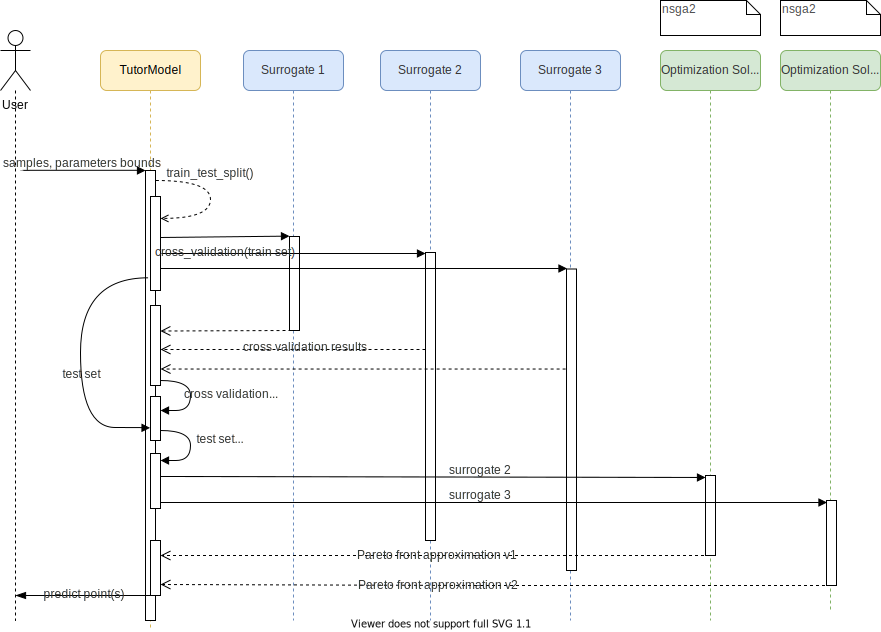
\includegraphics[width=\textwidth]{content/images/portfolio_validation_solv}
            \caption[Portfolio validation activity]{This is a validation and optimization workflow of several surrogates}
            \label{fig:tutor_activity}
        \end{figure}

    In the case of mixed surrogates models portfolio, validation pass in two groups: multi-objectives and single objective surrogates. In single-objective surrogates group must additionally restore complite hypotheisis for the multi-dimensional objective surface.


    \begin{enumerate}
        \item You have to try multiple types of surrogate(models) to find the best one for your data.
        \item A number of NFL theorems were derived that demonstrate the danger of comparing algorithms by their performance on a small sample of problems.
    \end{enumerate}

    As metamodel-based algorithms are generally developed for black box problems, where characteristics of the problems to be solved are not known a priori, one can measure the efficiency of an algorithm by its ability to provide meaningful solutions in a least number of function evaluations \cite{SoftSurvey}.

    A set of models is defined that can form a partial or complete hypothesis to describe the problem. Also during the increase of the experiments may change the model that best describes the existing problem As a result, there is variability for each problem and configuration step at the same time. A set of hypotheses can solve this problem but it takes longer time for cross validation.


    % ---------------------------------------------------        Sampling strategy
    \subsection{Sampling strategy} In many practical problems, only a restricted budget is spendable. Each evaluated point should be informative to reduce cost and improve interpolation by models. The most straightforward method of sampling design is a random witch for small sample sizes, often produce clusters of samples. 
    Alternatively, implemented Sobol sampling\cite{Sobol1999}, which covers the space more evenly. Out of the box, we provide Sobol sampling and random sampling.
    
    
    % Oversampling and undersampling in data analysis. Alleviate imbalance in the dataset. 
    % Imbalance in dataset is not always a problem, more so for optimization tasks. 

    % The main gain for models not to provide best accuracy on all search space but provide possible optimum regions.
    % Accuracy in prediction optimal regions or points from there will direct the search in the right direction.

    % Predictor variables can legitimately over- or under-sample. 
    % In this case, provided a carefully check that the model assumptions seem valid.

    % for other set of parameters, and make a choice from more diverse pool of models.

% --------------------------------------------------------------------------------------------
% ---------------------------------------------------       Solvers      
% --------------------------------------------------------------------------------------------
\section{Solvers}

    Optimization algorithms. MOEA. A Python platform\cite{francesco_biscani_2019}  to perform parallel computations of optimisation tasks (global and local) via the asynchronous generalized island model.

    decorators for single-objective solver with multi-objective surrogate 

    Solvers role is to apply an optimization algorithm on the surrogate and find a solution(s). Most solvers implemented with Multi-objective evolutionary algorithms such as NSGA2, MOEA/D, Multi-objective Ant Colony Optimizer (MACO) or Nondominated Sorting Particle Swarm Optimizer (NSPSO)\cite{francesco_biscani_2019}. 
    Specifically added solver with a combination of several multi-objective genetic algorithms with a shared population.

    Accordingly, on this step, a version of the solver with a scalarization of surrogates values possible witch optimize with any optimal heuristics. In this case, only one optimal point is obtained from the Pareto front, so the process must be repeated as many times as necessary to obtain the required count. 







% ----------    Designing a Sampling Plan
% \paragraph{Designing a Sampling Plan} The most straightforward way of sampling a design space in a uniform fashion is by \cite{EngSurMod} means of a rectangular grid of points. 
% Random sampling has the downside that for small sample sizes, there is often signficant clustering of samples, which is not ideal for interpolation since clustered samples can be wasteful. Instead, often a better option is to use a Latin hypercube, which enforces a condition that sample bins may not share the same coordinates for any coordinate axis







% Without automated tools, it can take days for experts to review just a few dozen examples.  In that same time, an automatic tool can explore thousands to millions to billions more solutions. People find it an overwhelming task just to certify the correctness of conclusions generated from so many results.


% Managing complex execution Strategies


% The simplifications are mean to discard the superfluous details that are unlikely to generalize to new instances. However, to decide what data to discard and what data to keep, you must make a hypothesis. For example, a linear model makes the hypothesis that the data is fundamentally linear and that the distance between the instances and the straight line is just noise, which can safely be ignored.